\RequirePackage[l2tabu, orthodox]{nag}
\documentclass[french,english]{beamer}
%INSTALL

%avoids a warning
\usepackage[log-declarations=false]{xparse}
\usepackage{fontspec} %font selecting commands
\usepackage{xunicode}
\usepackage{ucharclasses}
%warn about missing characters
\tracinglostchars=2

%REDAC
\usepackage{booktabs}
\usepackage{calc}
\usepackage{tabularx}

\usepackage{etoolbox} %for addtocmd, newtoggle commands
\newtoggle{LCpres}
\toggletrue{LCpres}

\usepackage{mathtools} %load this before babel!
	\mathtoolsset{showonlyrefs,showmanualtags}

%\usepackage[french, english]{babel}%options should probably be on the document level
\usepackage{babel}
%suppresses the warning about frenchb not modifying the captions (“—” to “:” in “Figure 1 – Legend”).
%	\frenchbsetup{AutoSpacePunctuation=false,SuppressWarning=true}% test with false?
	\frenchbsetup{AutoSpacePunctuation=false,SuppressWarning=false}

%\usepackage[super]{nth}%better use fmtcount! (loaded by datetime anyway; see below about pbl with warnings and package silence)
\usepackage{listings} %typeset source code listings
	\lstset{language=XML,tabsize=2,captionpos=b,basicstyle=\NoAutoSpacing}%NoAutoSpacing avoids space before colon or ?}%,literate={"}{{\tt"}}1, keywordstyle=\fontspec{Latin Modern Mono Light}\textbf, emph={String, PreparedStatement}, emphstyle=\fontspec{Latin Modern Mono Light}\textbf, language=Java, basicstyle=\small\NoAutoSpacing\ttfamily, aboveskip=0pt, belowskip=0pt, showstringspaces=false
\usepackage[nolist,smaller,printonlyused]{acronym}%,smaller option produces warnings from relsize in some cases, it seems.% Note silence and acronym and hyperref make (xe)latex crash when ac used in section (http://tex.stackexchange.com/questions/103483/strange-packages-interaction-acronyms-silence-hyperref), rather use \section{\texorpdfstring{\acs{UE}}{UE}}.
\usepackage{fmtcount}
\usepackage[nodayofweek]{datetime}%must be loaded after the babel package. However, loading it after {nth} generates a warning from fmtcount about ordinal being already defined. Better load it before nth? (then we can remove the silence package which creates possible crashes, see above.) Or remove nth?
%\usepackage{xspace}%do we need this?
\nottoggle{LCpres}{
	\usepackage[textsize=small]{todonotes}
}
\iftoggle{LCpres}{
	%remove pdfusetitle (implied by beamer)
	\usepackage{hyperref}
}{
% option pdfusetitle must be introduced here, not in hypersetup.
	\usepackage[pdfusetitle]{hyperref}
}
%breaklinks makes links on multiple lines into different PDF links to the same target.
%colorlinks (false): Colors the text of links and anchors. The colors chosen depend on the the type of link. In spite of colored boxes, the colored text remains when printing.
%linkcolor=black: this leaves other links in colors, e.g. refs in green, don't print well.
%pdfborder (0 0 1, set to 0 0 0 if colorlinks): width of PDF link border
%hidelinks
\hypersetup{breaklinks, bookmarksopen}
%add hyperfigures=true in hypersetup (already defined in article mode)
\iftoggle{LCpres}{
	\hypersetup{hyperfigures}
}

%in Beamer, sets url colored links but does not change the rest of the colors (http://tex.stackexchange.com/questions/13423/how-to-change-the-color-of-href-links-for-real)
%\hypersetup{breaklinks,bookmarksopen,colorlinks=true,urlcolor=blue,linkcolor=,hyperfigures=true}
% hyperref doc says: Package bookmark replaces hyperref’s bookmark organization by a new algorithm (...) Therefore I recommend using this package.
\usepackage{bookmark}

% center floats by default, but do not use with float
% \usepackage{floatrow}
% \makeatletter
% \g@addto@macro\@floatboxreset\centering
% \makeatother
\nottoggle{LCpres}{
	\usepackage{enumitem} %follow enumerate by a string saying how to display enumeration
}
\usepackage{ragged2e} %new com­mands \Cen­ter­ing, \RaggedLeft, and \RaggedRight and new en­vi­ron­ments Cen­ter, FlushLeft, and FlushRight, which set ragged text and are eas­ily con­fig­urable to al­low hy­phen­ation (the cor­re­spond­ing com­mands in LaTeX, all of whose names are lower-case, pre­vent hy­phen­ation al­to­gether). 
\usepackage{siunitx} %[expproduct=tighttimes, decimalsymbol=comma] ou (plus récent ?) [round-mode=figures, round-precision=2, scientific-notation = engineering]
\sisetup{detect-all, locale = FR, strict}% to detect e.g. when in math mode (use a math font) - check whether this makes sense with strict
\usepackage{braket} %for \Set
\usepackage{natbib}
\usepackage{doi}

\usepackage{amsmath,amsthm}
% \usepackage{amsfonts} %not required?
% \usepackage{dsfont} %for what?
%unicode-math overwrites the following commands from the mathtools package: \dblcolon, \coloneqq, \Coloneqq, \eqqcolon. Using the other colon-like commands from mathtools will lead to inconsistencies. Plus, Using \overbracket and \underbracke from mathtools package. Use \Uoverbracket and \Uunderbracke for original unicode-math definition.
%use exclusively \mathbf and choose math bold style below.
\usepackage[warnings-off={mathtools-colon, mathtools-overbracket}, bold-style=ISO]{unicode-math}

\defaultfontfeatures{
	Fractions=On,
	Mapping=tex-text% to turn "--" into dashes, useful for bibtex%%
}
%\defaultfontfeatures[\rmfamily, \sffamily]{
%\defaultfontfeatures[\rmfamily]{
%	Fractions=On,
%	Mapping=% to leave " alone (disable the default mapping tex-text; requires loading the font afterwards?)
%}
\newfontfamily\xitsfamily{XITS}
\newfontfamily\texgyretermesfamily{TeX Gyre Termes}
\newfontfamily\texgyreherosfamily{TeX Gyre Heros}
\newfontfamily\lmfamily{Latin Modern Roman}
\iftoggle{LCpres}{
	\setmainfont{Latin Modern Roman}
	\setsansfont{Latin Modern Sans}
	\setmonofont{Latin Modern Mono}
}{
	\setmainfont{TeX Gyre Termes}
	\setsansfont{TeX Gyre Heros}
	\setmonofont{TeX Gyre Cursor}
}
\defaultfontfeatures{}%disable default font features to avoid warnings with math fonts.
\setmathfont{XITS Math}
\setmathfont[range={\mathcal,\mathbfcal},StylisticSet=1]{XITS Math}
%to make \boldmath $\cdot$ work (otherwise: “Missing character: There is no ⋅ in font XITS Math Bold/OT:script=math;language =DFLT;!”). Alternative: \setmathfont[BoldFont=XITS Math]{XITS Math}
\setmathfont[range={"22C5},version=bold]{XITS Math}
%silently delays restoring normal font when using e.g. “≠)” or “≠ other word”.
%\setTransitionTo{Arrows}{\xitsfamily}
%\setTransitionTo{MathematicalOperators}{\xitsfamily}
%this solution explicitly fails on “≠)” and works for “≠ other word.”
\setTransitionsFor{MathematicalOperators}{\begingroup\xitsfamily}{\endgroup}
\setTransitionsFor{Arrows}{\begingroup\xitsfamily}{\endgroup}
%texgyretermes does not have ✓, XITS does.
\setTransitionsFor{Dingbats}{\begingroup\xitsfamily}{\endgroup}
%this also works, but it is more complex
%\def\ResetTransitionTo#1{%
%  \XeTeXinterchartoks 255 \csname#1Class\endcsname{\relax}}
%\setTransitionsFor{MathematicalOperators}
%  {\begingroup\ResetTransitionTo{MathematicalOperators}\xitsfamily}
%  {\endgroup}

\usepackage{cleveref}% cleveref should go "laster" than hyperref
%GRAPHICS
\usepackage{pgf}
\usepackage{pgfplots}
	\usetikzlibrary{babel, matrix, fit, plotmarks, calc, trees, shapes.geometric, positioning, plothandlers, arrows, shapes.multipart}
\pgfplotsset{compat=1.11}
\usepackage{graphicx}

\graphicspath{{graphics/},{graphics-dm/}}
\DeclareGraphicsExtensions{.pdf}
\LetLtxMacro\SavedIncludeGraphics\includegraphics
\AtBeginDocument{
	\def\includegraphics#1#{% #1 catches optional stuff (star/opt. arg.)
		\IncludeGraphicsAux{#1}%
	}%
}
\newcommand*{\IncludeGraphicsAux}[2]{%
	\XeTeXLinkBox{%
		\SavedIncludeGraphics#1{#2}%
	}%
}%

%HACKING
\usepackage{printlen}
\uselengthunit{mm}
% 	\newlength{\templ}% or LenTemp?
% 	\setlength{\templ}{6 pt}
% 	\printlength{\templ}
\usepackage{scrhack}% load at end. Corrects a bug in float package, which is outdated but might be used by other packages
\usepackage{xltxtra} %somebody said that this is loaded by fontspec, but does not seem correct: if not loaded explicitly, does not appear in the log and \showhyphens is not corrected.

%Beamer-specific
%do not remove babel, which beamer uses (beamer uses the \translate command for the appendix); but french can be removed.
\iftoggle{LCpres}{
	\usepackage{appendixnumberbeamer}
	\setbeamertemplate{navigation symbols}{} 
	\usepackage{preamble/beamerthemeParisFrance}
	\usefonttheme{professionalfonts}
	\setcounter{tocdepth}{10}
	%From: http://tex.stackexchange.com/questions/168057/beamer-with-xelatex-on-texlive2013-enumerate-numbers-in-black
%I don’t think it’s useful to submit this as a bug: nothing has been solved since March, 2015. See: https://bitbucket.org/rivanvx/beamer/issues?status=resolved.

\setbeamertemplate{enumerate item}
{
  \begin{pgfpicture}{-1ex}{-0.65ex}{1ex}{1ex}
    \usebeamercolor[fg]{item projected}
    {\pgftransformscale{1.75}\pgftext{\normalsize\pgfuseshading{bigsphere}}}
    {\pgftransformshift{\pgfpoint{0pt}{0.5pt}}
      \pgftext{\usebeamercolor[fg]{item projected}\usebeamerfont*{item projected}\insertenumlabel}}
  \end{pgfpicture}%
}

\setbeamertemplate{enumerate subitem}
{
  \begin{pgfpicture}{-1ex}{-0.55ex}{1ex}{1ex}
    \usebeamercolor[fg]{subitem projected}
    {\pgftransformscale{1.4}\pgftext{\normalsize\pgfuseshading{bigsphere}}}
    \pgftext{%
      \usebeamercolor[fg]{subitem projected}%
      \usebeamerfont*{subitem projected}%
      \insertsubenumlabel}
  \end{pgfpicture}%
}

\setbeamertemplate{enumerate subsubitem}
{
  \begin{pgfpicture}{-1ex}{-0.55ex}{1ex}{1ex}
    \usebeamercolor[fg]{subsubitem projected}
    {\pgftransformscale{1.4}\pgftext{\normalsize\pgfuseshading{bigsphere}}}
    \pgftext{%
      \usebeamercolor[fg]{subsubitem projected}%
      \usebeamerfont*{subitem projected}%
      \insertsubsubenumlabel}
  \end{pgfpicture}%
}


}
% \newcommand{\citep}{\cite}%Better: leave natbib.
% \setbeamersize{text margin left=0.1cm, text margin right=0.1cm} 
% \usetheme{BrusselsBelgium}%no, replace with paris
%\usetheme{ParisFrance}, no, usepackage better!
% Tex Gyre takes too much space, replace with Latin Modern Roman / Sans / Mono.
% Difference when loading explicitly Latin Modern Sans (compared to not using \setsansfont at all):
% the font LMSans17-Regular appears in the document;
% the title of the slides appears differently;
% it does not say (in the log file):
% > LaTeX Font Info:    Font shape `EU1/lmss/m/it' in size <10.95> not available
% > (Font)              Font shape `EU1/lmss/m/sl' tried instead on input line 85.
% > LaTeX Font Info:    Try loading font information for EU1+lmtt on input line 85.

%tikzposter-specific
%remove \usepackage{ragged2e}: causes 1=1 to be printed in the middle of the poster. (Anyway prints a warning about those characters being missing.)
%put [french, english] options next to \usepackage{babel} to avoid warning of 

\newcommand{\R}{ℝ}
\newcommand{\N}{ℕ}
\newcommand{\Z}{ℤ}
\newcommand{\card}[1]{\lvert{#1}\rvert}
\newcommand{\powerset}[1]{\mathscr{P}(#1)}%\mathscr rather than \mathcal: scr is rounder than cal (at least in XITS Math).
\newcommand{\suchthat}{\;\ifnum\currentgrouptype=16 \middle\fi|\;}
%\newcommand{\Rplus}{\reels^+\xspace}

\AtBeginDocument{%
	\renewcommand{\epsilon}{\varepsilon}
% we want straight form of \phi for mathematics, as recommended in UTR #25: Unicode support for mathematics.
%	\renewcommand{\phi}{\varphi}
}

% with amssymb, but I don’t want to use amssymb just for that.
% \newcommand{\restr}[2]{{#1}_{\restriction #2}}
%\newcommand{\restr}[2]{{#1\upharpoonright}_{#2}}
\newcommand{\restr}[2]{{#1|}_{#2}}%sometimes typed out incorrectly within \set.
%\newcommand{\restr}[2]{{#1}_{\vert #2}}%\vert errors when used within \Set and is typed out incorrectly within \set.
\DeclareMathOperator*{\argmax}{arg\,max}
\DeclareMathOperator*{\argmin}{arg\,min}


%Voting and MCDA
\newcommand{\allalts}{\mathscr{A}}
\newcommand{\alts}{A}
\newcommand{\allF}{\mathcal{F}}
\newcommand{\cat}[1]{C_{#1}}

%Voting
\newcommand{\feasalts}{F}
\newcommand{\allvoters}{\mathscr{N}}
\newcommand{\voters}{N}
\newcommand{\allsystems}{\mathcal{G}}
\newcommand{\prof}{\mathbf{R}}
\newcommand{\allprofs}{\mathbfcal{R}}
\newcommand{\linors}{\mathcal{L}(\alts)}

\newcommand{\pbasic}[1]{\prof^{#1}_\epsilon}
\newcommand{\pelem}[1]{\prof^{#1}_e}
\newcommand{\pcycl}[1]{\prof^{#1}_c}
\newcommand{\pcycllong}[1]{\prof^{#1}_{cl}}
\newcommand{\pinv}[1]{\overline{\prof_{#1}}}
\newcommand{\dmap}{{\xitsfamily δ}}
%powerset without zero
\newcommand{\powersetz}[1]{\mathcal{P}_\emptyset(#1)}

%logic atom
%⟼ (long)
\DeclareDocumentCommand{\lato}{ O{\prof} O{\alts} }{[#1 \!⟼\! #2]}
%logic atom in
%↝, \stackrel{\in}{\mapsto}, ➲, ⥹
\newcommand{\tightoverset}[2]{%
  \mathop{#2}\limits^{\vbox to -.5ex{\kern-0.9ex\hbox{$#1$}\vss}}}
\DeclareDocumentCommand{\latoin}{ O{\prof} O{\alpha} }{[#1 \tightoverset{\in}{⟼} #2]}
\newcommand{\alllang}{\mathcal{L}}
\newcommand{\ltru}{\texttt{T}}
\newcommand{\lfal}{\texttt{F}}
\newcommand{\laxiom}[1]{{\texgyreherosfamily{\textsc{#1}}}}

%ARG TH
\newcommand{\AF}{\mathcal{AF}}
\newcommand{\labelling}{\mathcal{L}}
\newcommand{\labin}{\textbf{in}\xspace}
\newcommand{\labout}{\textbf{out}}
\newcommand{\labund}{\textbf{undec}\xspace}
\newcommand{\nonemptyor}[2]{\ifthenelse{\equal{#1}{}}{#2}{#1}}
\newcommand{\gextlab}[2][]{
	\labelling{\mathcal{GE}}_{(#2, \nonemptyor{#1}{\ibeatsr{#2}})}
}
\newcommand{\allargs}{A^*}
\newcommand{\args}{A}
\newcommand{\ar}{a}
\newcommand{\ext}{\mathcal{E}}

%MCDA+Arg
\newcommand{\dm}{d}
\newcommand{\ileadsto}{\rightcurvedarrow}
\newcommand{\mleadsto}[1][\eta]{\rightcurvedarrow_{#1}}
\newcommand{\ibeats}{\vartriangleright}
\newcommand{\mbeats}[1][\eta]{\vartriangleright_{#1}}

%MISC
\newcommand{\lequiv}{\Vvdash}
\newcommand{\weightst}{W^{\,t}}

%MCDA classical
\newcommand{\crits}{\mathcal{J}}

%Sorting
\newcommand{\cats}{\mathcal{C}}
\newcommand{\catssubsets}{2^\cats}
\newcommand{\catgg}{\vartriangleright}
\newcommand{\catll}{\vartriangleleft}
\newcommand{\catleq}{\trianglelefteq}
\newcommand{\catgeq}{\trianglerighteq}
\newcommand{\alttoc}[2][x]{(#1 \xrightarrow{} #2)}
\newcommand{\alttocat}[3]{(#2 \xrightarrow{#1} #3)}
\newcommand{\alttoI}{(x \xrightarrow{} \left[\underline{C_x}, \overline{C_x}\right])}
\newcommand{\alttocatdm}[3][t]{\left(#2 \thinspace \raisebox{-3pt}{$\xrightarrow{#1}$}\thinspace #3\right)}
\newcommand{\alttocatatleast}[2]{\left(#1 \thinspace \raisebox{-3pt}{$\xrightarrow[]{≥}$}\thinspace #2\right)}
\newcommand{\alttocatatmost}[2]{\left(#1 \thinspace \raisebox{-3pt}{$\xrightarrow[]{≤}$}\thinspace #2\right)}

\definecolor{darkgreen}{rgb}{0,0.6,0}
\newcommand{\commentOC}[1]{{\selectlanguage{french}{\todo{OC : #1}}}}
%Or: \todo[color=green!40]
\newcommand{\innote}[1]{{\scriptsize{#1}}}

%this probably requires outdated float package, see doc KomaScript for an alternative.
% \newfloat{program}{t}{lop}
% \floatname{program}{PM}

%definition, theorem, lemma, example environments, qed trickery are only needed in article mode (not Beamer)
\nottoggle{LCpres}{
%style is plain by default (italic text)
	\newtheorem{definition}{Definition}
	\newtheorem{theorem}{Theorem}
%no italic: expected.
%http://tex.stackexchange.com/questions/144653/italicizing-of-amsthm-package
	\newtheorem{lemma}{Lemma}
%\crefname{axiom}{axiom}{axioms}%might be needed for workaround bug in cref when defining new theorems?

%\ifdefined\theorem\else
%\newtheorem{theorem}{\iflanguage{english}{Theorem}{Théorème}}
%\fi

\theoremstyle{remark}
	\newtheorem{examplex}{Example}
	\newtheorem{remarkx}{Remark}

%trickery allowing use of \qedhere and the like.
\newenvironment{example}{
	\pushQED{\qed}\renewcommand{\qedsymbol}{$\triangle$}\examplex
}{
	\popQED\endexamplex
}
\newenvironment{remark}{
	\pushQED{\qed}\renewcommand{\qedsymbol}{$\triangle$}\remarkx
}{
	\popQED\endremarkx
}
}
\crefname{examplex}{example}{examples}% I wonder why this is unnecessary in case of singular

%which line breaks are chosen: accept worse lines, therefore reducing risk of overfull lines. Default = 200
\tolerance=2000
%accept overfull hbox up to...
\hfuzz=2cm
%reduces verbosity about the bad line breaks
\hbadness 5000
%sloppy sets tolerance to 9999
\apptocmd{\sloppy}{\hbadness 10000\relax}{}{}

\bibliographystyle{abbrvnat}
%or \bibliographystyle{apalike} for presentations?

%doi package uses old-style dx.doi url, see 3.8 DOI system Proxy Server technical details, “Users may resolve DOI names that are structured to use the DOI system Proxy Server (http://doi.org (preferred) or http://dx.doi.org).”, https://www.doi.org/doi_handbook/3_Resolution.html
\makeatletter
\patchcmd{\@doi}{dx.doi.org}{doi.org}{}{}
\makeatother

% WRITING
%\newcommand{\ie}{i.e.\@\xspace}%to try
%\newcommand{\eg}{e.g.\@\xspace}
%\newcommand{\etal}{et al.\@\xspace}
\newcommand{\ie}{i.e.\ }
\newcommand{\eg}{e.g.\ }
\newcommand{\mkkOK}{\checkmark}%\color{green}{\checkmark}
\newcommand{\mkkREQ}{\ding{53}}%requires pifont?%\color{green}{\checkmark}
\newcommand{\mkkNO}{}%\text{\color{red}{\textsf{X}}}

\makeatletter
\newcommand{\boldor}[2]{%
	\ifnum\strcmp{\f@series}{bx}=\z@
		#1%
	\else
		#2%
	\fi
}
\newcommand{\textstyleElProm}[1]{\boldor{\MakeUppercase{#1}}{\textsc{#1}}}
\makeatother
\newcommand{\electre}{\textstyleElProm{Électre}\xspace}
\newcommand{\electreIv}{\textstyleElProm{Électre Iv}\xspace}
\newcommand{\electreIV}{\textstyleElProm{Électre IV}\xspace}
\newcommand{\electreIII}{\textstyleElProm{Électre III}\xspace}
\newcommand{\electreTRI}{\textstyleElProm{Électre Tri}\xspace}
% \newcommand{\utadis}{\texorpdfstring{\textstyleElProm{utadis}\xspace}{UTADIS}}
% \newcommand{\utadisI}{\texorpdfstring{\textstyleElProm{utadis i}\xspace}{UTADIS I}}

%TODO
% \newcommand{\textstyleElProm}[1]{{\rmfamily\textsc{#1}}} 


%const
\newcommand{\tikzboxit}{\path node[draw, overlay, inner sep=0.6mm, fit=(boxed), rectangle] {};}%

\newlength{\GraphsNodeSep}
\setlength{\GraphsNodeSep}{7mm}

% MCDA Drawing Sorting
\newlength{\MCDSCatHeight}
\setlength{\MCDSCatHeight}{6mm}
\newlength{\MCDSAltHeight}
\setlength{\MCDSAltHeight}{4mm}
%separation between two vertical alts
\newlength{\MCDSAltSep}
\setlength{\MCDSAltSep}{2mm}
\newlength{\MCDSCatWidth}
\setlength{\MCDSCatWidth}{3cm}
\newlength{\MCDSAltWidth}
\setlength{\MCDSAltWidth}{2.5cm}
\newlength{\MCDSEvalRowHeight}
\setlength{\MCDSEvalRowHeight}{6mm}
\newlength{\MCDSAltsToCatsSep}
\setlength{\MCDSAltsToCatsSep}{1.5cm}
\newcounter{MCDSNbAlts}
\newcounter{MCDSNbCats}
\newlength{\MCDSArrowDownOffset}
\setlength{\MCDSArrowDownOffset}{0mm}

\tikzset{/Graphs/dot/.style={
	shape=circle, fill=black, inner sep=0, minimum size=1mm
}}
\tikzset{/MC/D/S/alt/.style={
	shape=rectangle, draw=black, inner sep=0, minimum height=\MCDSAltHeight, minimum width=\MCDSAltWidth
}}
\tikzset{MC/D/S/pref/.style={
	shape=ellipse, draw=gray, thick
}}
\tikzset{/MC/D/S/cat/.style={
	shape=rectangle, draw=black, inner sep=0, minimum height=\MCDSCatHeight, minimum width=\MCDSCatWidth
}}
\tikzset{/MC/D/S/evals matrix/.style={
	matrix, row sep=-\pgflinewidth, column sep=-\pgflinewidth, nodes={shape=rectangle, draw=black, inner sep=0mm, text depth=0.5ex, text height=1em, minimum height=\MCDSEvalRowHeight, minimum width=12mm}, nodes in empty cells, matrix of nodes, inner sep=0mm, outer sep=0mm, row 1/.style={nodes={draw=none, minimum height=0em, text height=, inner ysep=1mm}}
}}

\newlength{\GitCommitSep}
\setlength{\GitCommitSep}{13mm}

\tikzset{/Git/commit/.style={
	shape=rectangle, draw, minimum width=4em, minimum height=0.6cm
}}
\tikzset{/Git/branch/.style={
	shape=ellipse, draw, red
}}
\tikzset{/Git/head/.style={
	shape=ellipse, draw, fill=yellow
}}

\tikzset{profile matrix/.style={
	matrix of math nodes, column sep=3mm, row sep=2mm, nodes={inner sep=0.5mm, anchor=base}
}}
\tikzset{rank-profile matrix/.style={
	matrix of math nodes, column sep=3mm, row sep=2mm, nodes={anchor=base}, column 1/.style={nodes={inner sep=0.5mm}}, row 1/.style={nodes={inner sep=0.5mm}}
}}
\tikzset{rank-vector/.style={
	draw, rectangle, inner sep=0, outer sep=1mm
}}
\tikzset{isolated rank-vector/.style={
	draw, matrix of math nodes, column sep=3mm, inner sep=0, matrix anchor=base, nodes={anchor=base, inner sep=.33em}, ampersand replacement=\&
}}

% GUI
\tikzset{/GUI/button/.style={
	rectangle, very thick, rounded corners, draw=black, fill=black!40%, top color=black!70, bottom color=white
}}

% Logger objects
\tikzset{/logger/main/.style={
	shape=rectangle, draw=black, inner sep=1ex, minimum height=7mm
}}
\tikzset{/logger/helper/.style={
	shape=rectangle, draw=black, dashed, minimum height=7mm
}}
\tikzset{/logger/helper line/.style={
	<->, draw, dotted
}}

% Beliefs
\tikzset{/Beliefs/D/S/attacker/.style={
	shape=rectangle, draw, minimum size=8mm
}}
\tikzset{/Beliefs/D/S/supporter/.style={
	shape=circle, draw
}}

\newcommand{\tikzmark}[1]{%
	\tikz[overlay, remember picture, baseline=(#1.base)] \node (#1) {};%
}


\begin{acronym}
\acro{AMCD}{Aide Multicritère à la Décision}
\acro{ASA}{Argument Strength Assessment}
\acro{DA}{Decision Analysis}
\acro{DM}{Decision Maker}
\acro{DPr}{Deliberated Preferences}
\acro{DRSA}{Dominance-based Rough Set Approach}
\acro{DSS}{Decision Support Systems}
\acrodefplural{DSS}{Decision Support Systems}
% \newacroplural{DSS}[DSSes]{Decision Support Systems}
\acro{EJOR}{European Journal of Operational Research}
\acro{LNCS}{Lecture Notes in Computer Science}
\acro{MCDA}{Multicriteria Decision Aid}
\acro{MIP}{Mixed Integer Program}
\acro{NCSM}{Non Compensatory Sorting Model}
\acro{PL}{Programme Linéaire}
\acro{PLNE}{Programme Linéaire en Nombres Entiers}
\acro{PM}{Programme Mathématique}
\acro{MP}{Mathematical Program}
\acro{MIP}{Mixed Integer Program}
% \newacroplural{PM}{Programmes Mathématiques}
%acrodefplural since version 1.35, my debian has \ProvidesPackage{acronym}[2009/01/25, v1.34, Support for acronyms (Tobias Oetiker)]
\acrodefplural{PM}{Programmes Mathématiques}
\acro{PMML}{Predictive Model Markup Language}
\acro{RESS}{Reliability Engineering \& System Safety}
\acro{SMAA}{Stochastic Multicriteria Acceptability Analysis}
\acro{URPDM}{Uncertainty and Robustness in Planning and Decision Making}
\acro{XML}{Extensible Markup Language}
\end{acronym}


\title{Multicriteria Decision Aid}
\subtitle{A short introduction}
\subject{MCDA}
\keywords{subjectivity, preference elicitation, multiple criteria}
\author{Olivier Cailloux}
\institute[LAMSADE]{LAMSADE, Université Paris-Dauphine}
\date{\formatdate{18}{4}{2017}}

\setbeamertemplate{headline}[singleline]

\begin{document}
\begin{frame}[plain]
	\tikz[remember picture,overlay]{
		\path (current page.south west) node[anchor=south west, inner sep=0] {
			
\includegraphics[height=1cm]{LAMSADE95.jpg}
		};
		\path (current page.south) ++ (0, 1mm) node[anchor=south, inner sep=0] {
			
\includegraphics[height=9mm]{Dauphine.jpg}
		};
		\path (current page.south east) node[anchor=south east, inner sep=0] {
			
\includegraphics[height=1cm]{PSL.png}
		};
		\path (current page.south) ++ (0, 4em) node[anchor=south, inner sep=0] {
			\scriptsize\url{https://github.com/oliviercailloux/introduction-mcda}
		};
	}
	\titlepage
\end{frame}
\addtocounter{framenumber}{-1}

\begin{frame}
	\frametitle{Outline}
	\tableofcontents[subsectionstyle=hide]
\end{frame}

\section{Goal}
\begin{frame}
	\frametitle{Goal of \ac{MCDA}}
	Desired:
	\begin{itemize}
		\item decide in agreement with your own preferences
		\item in a systematic way
	\end{itemize}
	Preferences: intuitive knowledge of what’s right for you
	\begin{block}{One goal of \ac{MCDA}}
		Model preferences
	\end{block}
\end{frame}

\begin{frame}
	\frametitle{\ac{MCDA}: what for? (Philosophically)}
	\centering
	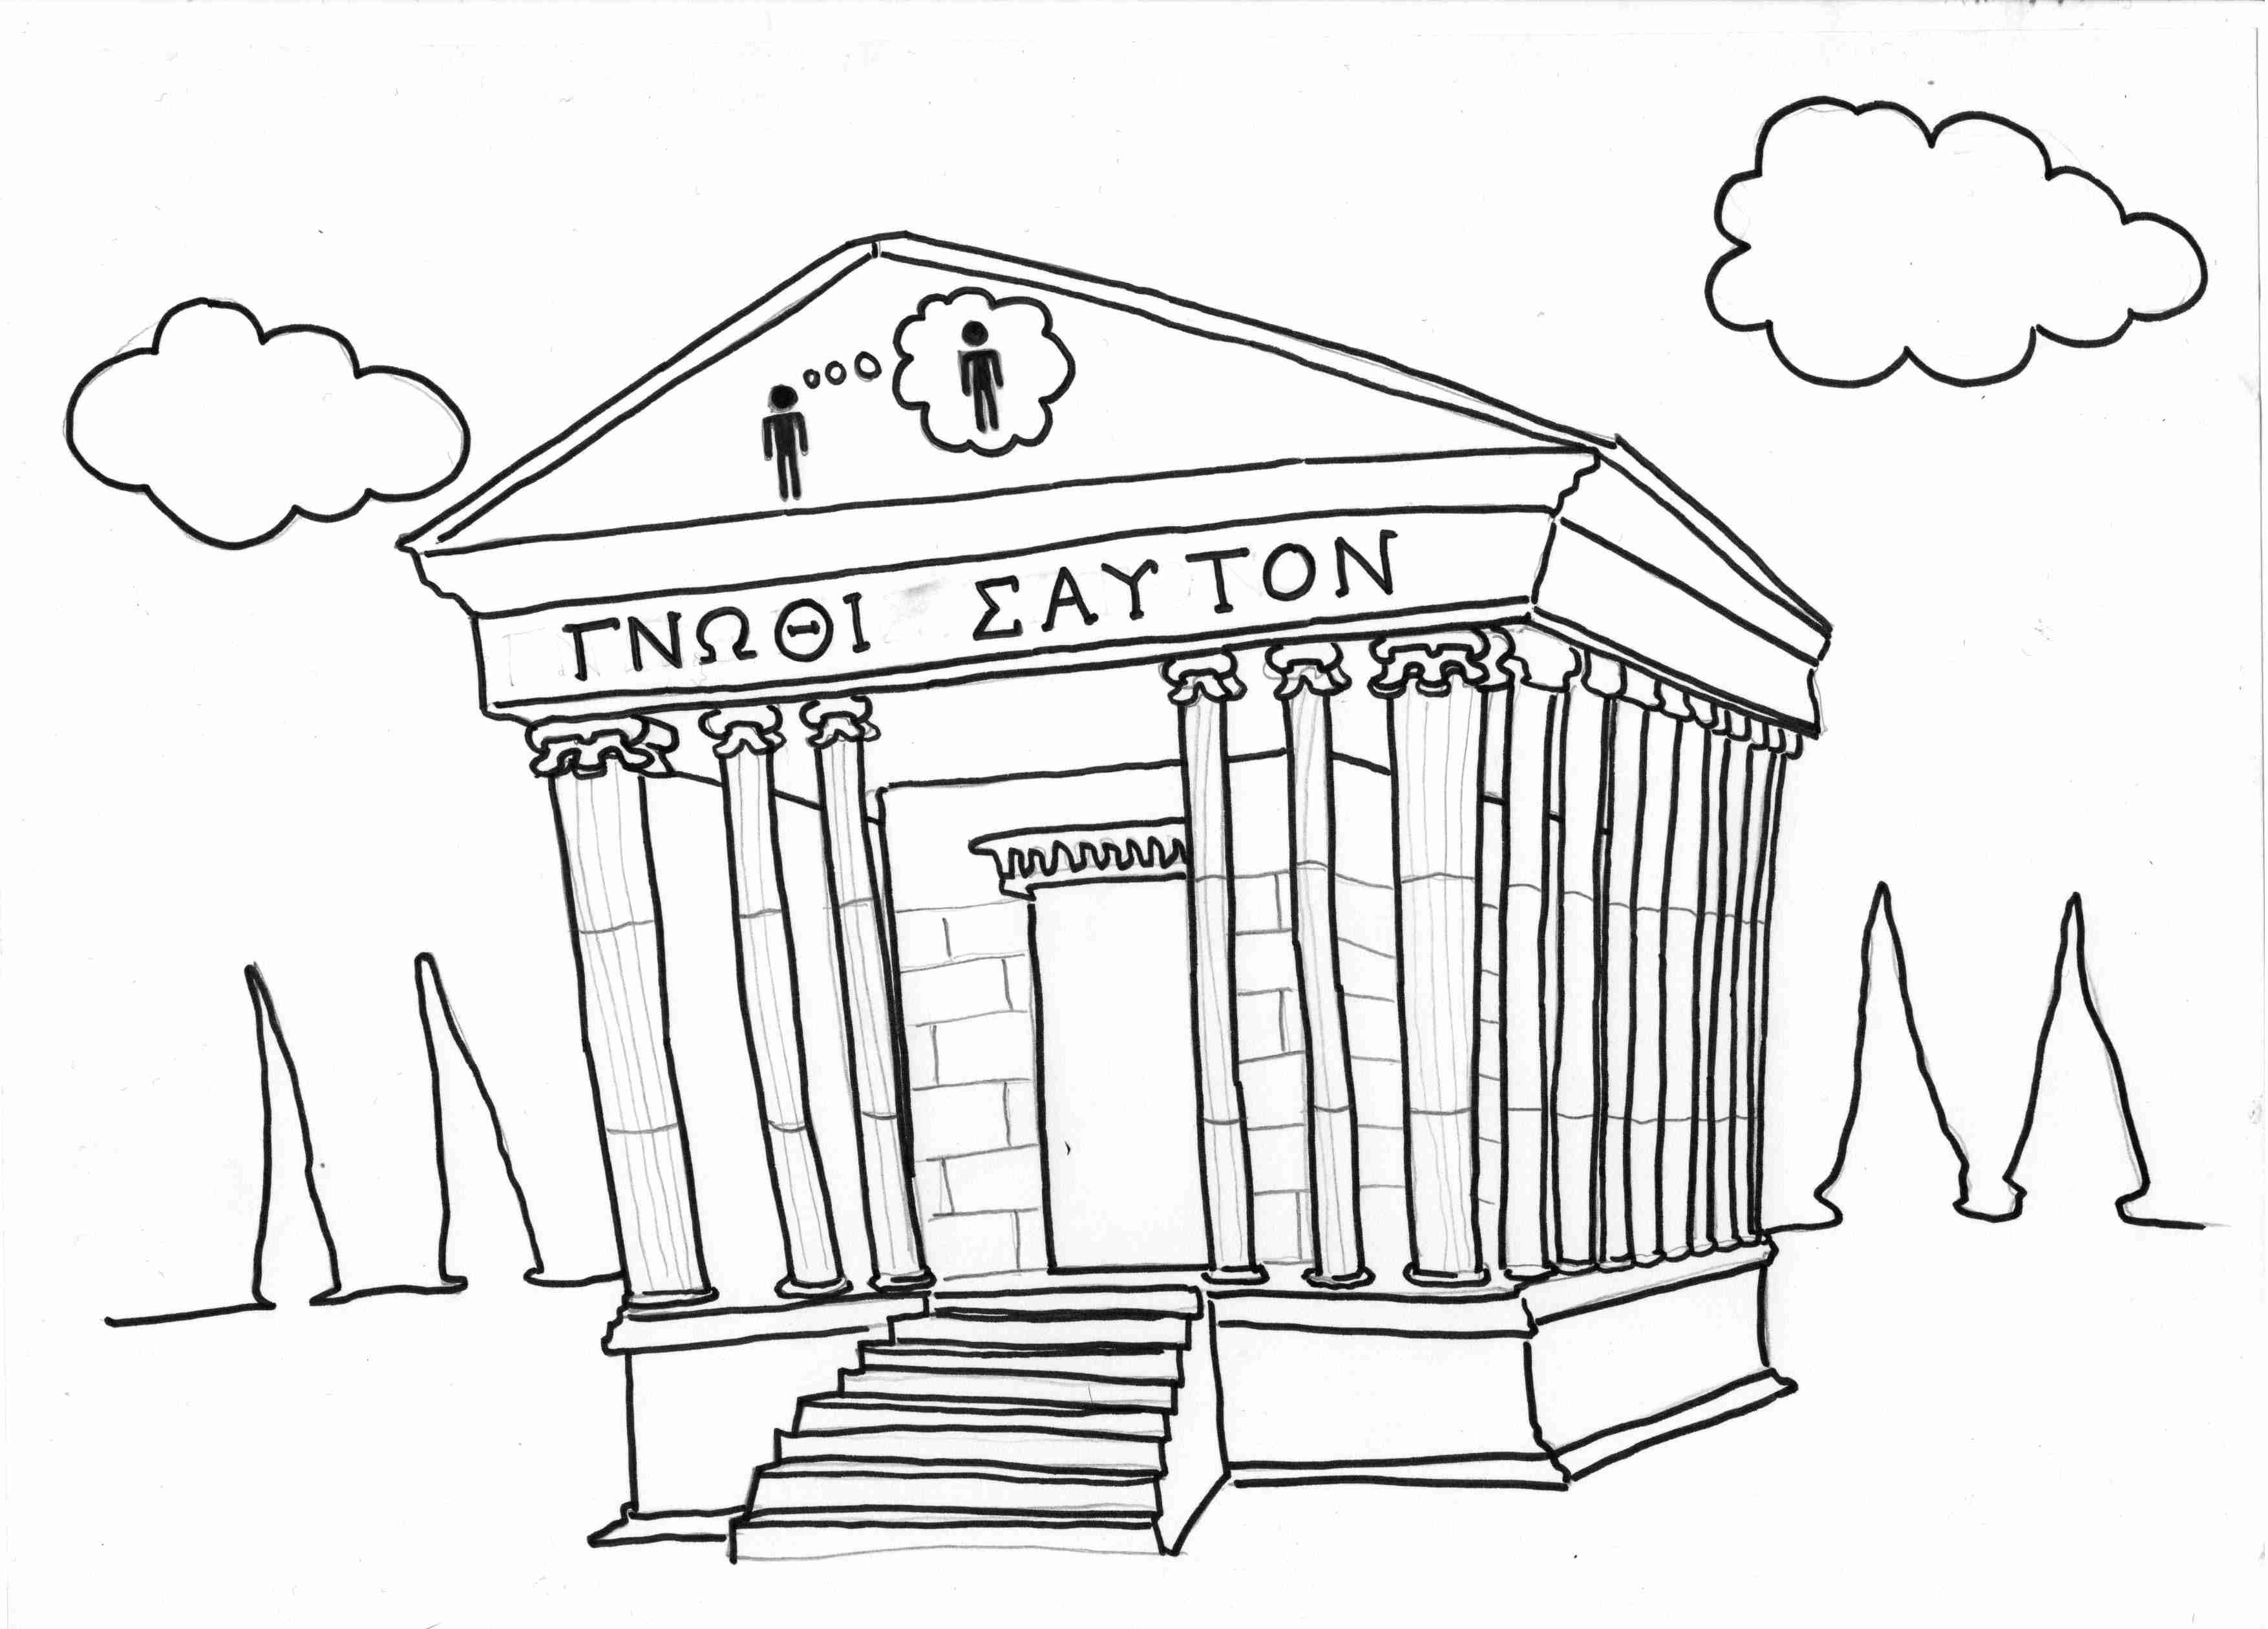
\includegraphics[height=5cm]{ConnaisToi20.jpg}
	\begin{block}{A Delphic maxim (Temple of Apollo)}
	\centering
		“Know thyself”
	\end{block}
\end{frame}

\begin{frame}
	\frametitle{\ac{MCDA}: what for? (More practically)}
	\begin{itemize}
		\item Make sure you take the right decision (for you)
		\item Discuss your intuitions
		\item Model expertise
		\item Understand intuitive notions (such as justice)
		\item Delegate decision making
	\end{itemize}
\end{frame}

\begin{frame}
	\frametitle{Why model preferences?}
	
	\begin{quote}
		There are three things extremely hard: Steel, a Diamond, and to know one's self.
	\end{quote}
	{\scriptsize\vspace{-2em}
	\begin{flushright}
%		B. \citeauthor{franklin_poor_2004} \citetext{[1800] \citeyear[p. 179]{franklin_poor_2004}}
		B. \citet[p. 179]{franklin_poor_2004}
	\end{flushright}
	}
	\begin{itemize}
		\item We hardly know our own preferences
		\item You can’t have everything
		\item Which trade-offs will you agree with?
	\end{itemize}
\end{frame}

\begin{frame}
	\frametitle{An example}
	\begin{itemize}
		\item Let’s choose what to plant in our garden
		\item Each year the performances change
		\item We want a systematic decision procedure
	\end{itemize}
	\begin{center}
		\begin{tikzpicture}
			\path node[matrix of nodes, ampersand replacement=\&] (my matrix) {
					\& quantity	\& taste	\& \node[align=left] {supports\\pollinators};	\& \node[align=left] {resists\\to cold};\\
				Tomatoes	\& 7	\& A	\& A	\& | (st 1) | −−\\
				Corn	\& 1.5	\& B	\& D	\& | (st 2) | −−\\
				Cabbage	\& 7.5	\& D	\& B	\& | (st 3) | ++\\
				Potatoes	\& 2.5	\& C	\& C	\& | (st 4) | +\\
				...	\& 	\& 	\& 	\& \\
			};
		\end{tikzpicture}
	\end{center}
\end{frame}

\section{Context}
\begin{frame}
	\frametitle{Context}
	\begin{itemize}
		\item Criteria $\crits$, scales $X_j, \forall j \in \crits$
		\item Action $a \in \prod_{j \in \crits} X_j$ is a vector of performances
		\item Action $\allalts = \prod_{j \in \crits} X_j$
		\item Available actions this year $\alts \subseteq \allalts$
		\item Winners this year $B \subseteq \alts$
	\end{itemize}
	\begin{block}{Goal}
		Obtain $f$ which maps any $A \subseteq \allalts$ to some $B \subseteq A$
	\end{block}
	\begin{center}
		\begin{tikzpicture}
			\path node[matrix of nodes, ampersand replacement=\&] (my matrix) {
					\& quantity	\& taste	\& \node[align=left] {sup. pollinators};	\& \node[align=left] {res. to cold};\\
				Tomatoes	\& 7	\& A	\& A	\& | (st 1) | −−\\
				Corn	\& 1.5	\& B	\& D	\& | (st 2) | −−\\
				Cabbage	\& 7.5	\& D	\& B	\& | (st 3) | ++\\
				Potatoes	\& 2.5	\& C	\& C	\& | (st 4) | +\\
			};
		\end{tikzpicture}
	\end{center}
\end{frame}

\begin{frame}
	\frametitle{Informational basis to determine $f$}
	\begin{itemize}
		\item We do \emph{not} search for the absolute best $f$
		\item $f$ models the \emph{preference}
		\item Of a decision maker
		\item Her subjectivity is to be integrated in $f$
	\end{itemize}
\end{frame}

\section[Preference]{What’s a preference?}
\begin{frame}
	\frametitle{What does “preferred” mean?}
	Let’s determine your “preferred” university
	\begin{itemize}
		\item Help a researcher choose her university?
		\item Help a student choose his university?
		\item Help government spread funding?
	\end{itemize}
\end{frame}

\begin{frame}
	\frametitle{Preference in MCDA}
	\begin{itemize}
		\item A decision problem
		\item A decision maker
		\item Preference {\tiny typically} defined in terms of \emph{desired action}
	\end{itemize}
\end{frame}

\begin{frame}
	\frametitle{Descriptive or prescriptive perspective}
	MCDA {\tiny typically} adopts a {\tiny weak} prescriptive perspective
	\begin{block}{Descriptive perspective}
		The model describes the “usual” behavior of the subjects
		\begin{itemize}
			\item Example: which drink does the subject buy?
			\item Predictive model
		\end{itemize}
	\end{block}
	\begin{block}{Prescriptive perspective}
		The model recommends actions coherent with the values of the \ac{DM}
		\begin{itemize}
			\item Example: you might want to consider this drink
			\item Possibly talk about hypothetical decisions
			\item Different validation
		\end{itemize}
	\end{block}
\end{frame}

\section{Methods}
\begin{frame}
	\frametitle{MCDA methods}
	\begin{itemize}
		\item $f$: a preference model (here, a strategy of choice)
		\item $f$ represents the subjectivity of the \ac{DM}
		\item $f$ maps $\alts \subseteq \allalts$ to $B \subseteq \alts$
		\item $\allF$ the set of possible functions
		\item How do we determine $f \in \allF$?
	\end{itemize}
	\begin{block}{MCDA method}
		\begin{itemize}
			\item Defines a class of functions $F \subseteq \allF$
			\item Together with a class of \emph{preferential parameters} $\Omega$
			\item Bijection maps $\omega \in \Omega$ to $f \in F$
		\end{itemize}
	\end{block}
%	(Parameterized) \emph{method}: a class of function
\end{frame}

\begin{frame}
	\frametitle{The Weighted sum method}
	\begin{itemize}
		\item Class of functions $F_\text{weighted sum}$: those that sum performances and compare the resulting scores
		\item Preference model $\omega$: a set of weights
		\item $\omega = \{w_j \in \R, \text{for each criterion }j\}$
		\item $f_\omega$ compares the weighted sums
	\end{itemize}
	Weights: $\omega = \left<0.3, 0.3, 0.2, 0.2\right>$
	\begin{center}
		\begin{tikzpicture}
			\path node[matrix of nodes, ampersand replacement=\&, inner sep=0, nodes={inner sep=.3333em}] (my matrix) {
					\& quantity	\& taste	\& \node[align=left] {supports\\pollinators};	\& \node[align=left] {resists\\to cold};\\
				Tomatoes	\& 7	\& 10	\& 7	\& | (st 1) | 0\\
				Corn	\& 1.5	\& 5	\& 1	\& | (st 2) | 0\\
				Cabbage	\& 7.5	\& 2	\& 5	\& | (st 3) | 10\\
				Potatoes	\& 2.5	\& 3	\& 3	\& | (st 4) | 5\\
			};
			\onslide<2>{\path (st 1 -| my matrix.east) ++ (20mm, 0) node[anchor=west] (sc 1) {6.5};}
			\onslide<1>{\path (st 1 -| my matrix.east) ++ (20mm, 0) node[anchor=west] (sc 1) {?};}
			\draw[->] (st 1 -| my matrix.east) -- (sc 1);
			\path (sc 1.west) ++(-10mm, 0.3cm) node (label) {$f_\omega$};
			\onslide<2>{\path (st 2 -| my matrix.east) ++ (20mm, 0) node[anchor=west] (sc 2) {2.15};}
			\draw[->] (st 2 -| my matrix.east) -- (sc 2);
			\onslide<2>{\path (st 3 -| my matrix.east) ++ (20mm, 0) node[anchor=west] (sc 3) {5.85};}
			\draw[->] (st 3 -| my matrix.east) -- (sc 3);
			\onslide<2>{\path (st 4 -| my matrix.east) ++ (20mm, 0) node[anchor=west] (sc 4) {3.25};}
			\draw[->] (st 4 -| my matrix.east) -- (sc 4);
		\end{tikzpicture}
	\end{center}
\end{frame}

\begin{frame}
	\frametitle{A problem with the weighted sum}
	The $f$ you want may not be in $F_\text{weighted sum}$
	\begin{itemize}
		\item You prefer St 1 to the other two?
		\item Score(St 1) > score(St 2) requires $w_\text{course 1} > w_\text{course 2}$
		\item Score(St 1) > score(St 3) requires $w_\text{course 2} > w_\text{course 1}$
	\end{itemize}
	\begin{center}
		\begin{tikzpicture}
			\path node[matrix of nodes, ampersand replacement=\&] (my matrix) {
					\& course 1	\& course 2\\
				St 1	\& 14	\& | (st 1) | 14\\
				St 2	\& 8	\& | (st 2) | 20\\
				St 3	\& 20	\& | (st 3) | 8\\
			};
			\path (st 1 -| my matrix.east) ++ (20mm, 0) node[anchor=west] (sc 1) {};
			\draw[->] (st 1 -| my matrix.east) -- (sc 1);
			\path (sc 1.west) ++(-10mm, 0.3cm) node (label) {$f_\omega$};
			\path (st 2 -| my matrix.east) ++ (20mm, 0) node[anchor=west] (sc 2) {};
			\draw[->] (st 2 -| my matrix.east) -- (sc 2);
			\path (st 3 -| my matrix.east) ++ (20mm, 0) node[anchor=west] (sc 3) {};
			\draw[->] (st 3 -| my matrix.east) -- (sc 3);
		\end{tikzpicture}
	\end{center}
\end{frame}

\section{Preference elicitation}
\begin{frame}
	\frametitle{Goal of preference elicitation}
	\begin{itemize}
		\item Assume we chose the method
		\item Method determines class of functions $F$ and class of parameters $\Omega$
		\item How shall we determine parameters $\omega \in \Omega$?
		\item The \ac{DM} does not know the answer
		\item Her usual behavior does not determine the answer
		\item BUT we assume she is available to answer questions
	\end{itemize}
\end{frame}

\begin{frame}
	\frametitle{Elicitation}
	\begin{block}{Elicit (\emph{Oxford English Dictionary}{\tiny , excerpt})}
		\begin{enumerate}
			\item To draw forth (what is latent or potential) into sensible existence.
			\item to extract, draw out (information) from a person by interrogation
			\item  To draw forth, evoke (a response, manifestation, etc.) from a person.
		\end{enumerate}
		\begin{quote}
			The edge of one [fissure] which elicited other sentiments than those of admiration.
		\end{quote}\vspace{-2em}\scriptsize
		\begin{flushright}
			J. Tyndall, Glaciers of Alps, i. §25. 188
		\end{flushright}
	\end{block}
	\begin{quote}
%		Ce raisin que le soleil élicite de la terre et que son rayon amical conduit de la fleur à la grappe (Claudel, Un Poète regarde la Croix, 1938, p. 128), Trésor de la langue française.
	\end{quote}
\end{frame}

\begin{frame}
	\frametitle{Preference elicitation}
	\begin{itemize}
		\item Ask questions to the \ac{DM}
		\item Questions must be: understandable
		\item Interpretable rigorously
		\item Informative
		\item {\tiny Hopefully} questions that the \ac{DM} can answer confidently
	\end{itemize}
	Goal: obtain a “satisfactory” $f$
	\begin{itemize}
		\item Elicitation can be: by parameters, by examples, or a mix, possibly using axiomatization
	\end{itemize}
\end{frame}

\begin{frame}
	\frametitle{Elicitation by parameters}
	\begin{itemize}
		\item Assume a method has three parameters with identifiable “roles”
		\item Explain the effects of the parameters on $f$
		\item Ask the \ac{DM} to fix the parameters
		\item Also permits to check whether the \ac{DM} accepts the method (accepts $F$)
		\item Possibly: show the effects of $f$ on samples
	\end{itemize}
\end{frame}

\begin{frame}
	\frametitle{Elicitation by examples}
	\begin{itemize}
		\item Use a set of examples to constrain $f$
		\item The \ac{DM} declares that $f$ should satisfy $f(\{a, b\}) = \{a\}$
		\item Sometimes: use historic examples
		\item Ideally these should be examples the \ac{DM} knows how to treat
		\item Detect whether some $f \in F$ represents all examples
	\end{itemize}
\end{frame}

\begin{frame}
	\frametitle{Axiomatic elicitation}
	\begin{itemize}
		\item A method can be axiomatized
		\item {\tiny Sometimes} means that we know exactly which questions to ask, in which sequence, to determine $f$
		\item And the conditions under which $f$ exists coherent with those answers
		\item May be compatible with other two approaches
	\end{itemize}
\end{frame}

\begin{frame}
	\frametitle{Some topics of study}
	\begin{itemize}
		\item (Axiomatic) study of classes of functions
		\item Elicitation procedures
		\item Extend to group decision making
		\item Extend to uncertainty on performances
		\item Cases study
	\end{itemize}
\end{frame}

\section{Open questions}
\begin{frame}
	\frametitle{Open questions}
	Is the model $f$ we obtain necessary?
	\begin{itemize}
		\item Several reasonable models may be possible
		\item What’s the part of arbitrariness in the model?
	\end{itemize}
	Will the \ac{DM} possibly accept (somehow) unreasonable models?
	\begin{itemize}
		\item What does unreasonable mean?
	\end{itemize}
	How do we compare models?
	\begin{itemize}
		\item How do we validate?
		\item What does $f$ model precisely?
	\end{itemize}
	Elicitation: are we asking questions the \ac{DM} can answer?
%K&T: framing effects. Slovic, Lability. We want the non-arbitrary part of the preferences
\end{frame}

\begin{frame}[plain]
	\addtocounter{framenumber}{-1}
	\begin{center}
		\huge
		\textit{Thank you for your attention!}
	\end{center}
\end{frame}

\appendix
\AtBeginSection{
}

\clearpage\pdfbookmark[2]{\refname}{\refname}
\begin{frame}
	\frametitle{\refname}
 	\bibliography{mcda}
\end{frame}

\clearpage\pdfbookmark{License}{License}
\begin{frame}[plain]
	\frametitle{License}
	This presentation, and the associated \LaTeX{} code, are published under the \href{http://opensource.org/licenses/MIT}{MIT license}. Feel free to reuse (parts of) the presentation, under condition that you cite the author.
	
	Credits are to be given to \href{http://www.lamsade.dauphine.fr/~ocailloux/}{Olivier Cailloux}, Université Paris-Dauphine.
	
	The drawing of the Temple of Apollo is copyrighted by Stéphane Deparis (used with permission). Many thanks to him.
\end{frame}
\addtocounter{framenumber}{-1}
\end{document}

\begin{frame}
	\frametitle{}
	\begin{itemize}
		\item 
	\end{itemize}
\end{frame}

\begin{frame}
	\frametitle{}
	\begin{block}{}
		\begin{itemize}
			\item 
		\end{itemize}
	\end{block}
\end{frame}
\end{document}
